%%%%%%%%%%%%%%%%%%%%%%%%%%%%%%%%%%%%%%%%%%%%%%%%%%%%%%%%%%%%%%%%%%%%%%%%%%%%
% AGUJournalTemplate.tex: this template file is for articles formatted with LaTeX
%
% This file includes commands and instructions
% given in the order necessary to produce a final output that will
% satisfy AGU requirements, including customized APA reference formatting.
%
% You may copy this file and give it your
% article name, and enter your text.
%
%
% Step 1: Set the \documentclass
%
%

%% To submit your paper:
\documentclass[draft]{agujournal2019}
\usepackage{url} %this package should fix any errors with URLs in refs.
\usepackage{lineno}
\usepackage[inline]{trackchanges} %for better track changes. finalnew option will compile document with changes incorporated.
\usepackage{soul}
\usepackage[version=4]{mhchem}
%\usepackage{natbib}

\linenumbers
%%%%%%%
% As of 2018 we recommend use of the TrackChanges package to mark revisions.
% The trackchanges package adds five new LaTeX commands:
%
%  \note[editor]{The note}
%  \annote[editor]{Text to annotate}{The note}
%  \add[editor]{Text to add}
%  \remove[editor]{Text to remove}
%  \change[editor]{Text to remove}{Text to add}
%
% complete documentation is here: http://trackchanges.sourceforge.net/
%%%%%%%

\draftfalse

%% Enter journal name below.
%% Choose from this list of Journals:
%
% JGR: Atmospheres
% JGR: Biogeosciences
% JGR: Earth Surface
% JGR: Oceans
% JGR: Planets
% JGR: Solid Earth
% JGR: Space Physics
% Global Biogeochemical Cycles
% Geophysical Research Letters
% Paleoceanography and Paleoclimatology
% Radio Science
% Reviews of Geophysics
% Tectonics
% Space Weather
% Water Resources Research
% Geochemistry, Geophysics, Geosystems
% Journal of Advances in Modeling Earth Systems (JAMES)
% Earth's Future
% Earth and Space Science
% Geohealth
%
% ie, \journalname{Water Resources Research}

\journalname{Geophysical Research Letters}


\begin{document}

%% ------------------------------------------------------------------------ %%
%  Title
%
% (A title should be specific, informative, and brief. Use
% abbreviations only if they are defined in the abstract. Titles that
% start with general keywords then specific terms are optimized in
% searches)
%
%% ------------------------------------------------------------------------ %%



\title{Antarctic Radiative and Temperature responses to a doubling of $\text{CO}_2$}

%% ------------------------------------------------------------------------ %%
%
%  AUTHORS AND AFFILIATIONS
%
%% ------------------------------------------------------------------------ %%

% Authors are individuals who have significantly contributed to the
% research and preparation of the article. Group authors are allowed, if
% each author in the group is separately identified in an appendix.)

% List authors by first name or initial followed by last name and
% separated by commas. Use \affil{} to number affiliations, and
% \thanks{} for author notes.
% Additional author notes should be indicated with \thanks{} (for
% example, for current addresses).

% Example: \authors{A. B. Author\affil{1}\thanks{Current address, Antartica}, B. C. Author\affil{2,3}, and D. E.
% Author\affil{3,4}\thanks{Also funded by Monsanto.}}

\authors{Lyssa M. Freese\affil{1}~ and Timothy W. Cronin\affil{1}}

 \affiliation{1}{Department of Earth, Atmosphere and Planetary Sciences, Massachusetts Institute of Technology}
% \affiliation{2}{Second Affiliation}
% \affiliation{3}{Third Affiliation}
% \affiliation{4}{Fourth Affiliation}

\affiliation{1}{Cambridge, Massachusetts, USA}
%(repeat as many times as is necessary)

%% Corresponding Author:
% Corresponding author mailing address and e-mail address:

% (include name and email addresses of the corresponding author.  More
% than one corresponding author is allowed in this LaTeX file and for
% publication; but only one corresponding author is allowed in our
% editorial system.)

% Example: \correspondingauthor{First and Last Name}{email@address.edu}

\correspondingauthor{L. M. Freese}{emfreese@mit.edu}

%% Keypoints, final entry on title page.

%  List up to three key points (at least one is required)
%  Key Points summarize the main points and conclusions of the article
%  Each must be 100 characters or less with no special characters or punctuation and must be complete sentences

% Example:
% \begin{keypoints}
% \item	List up to three key points (at least one is required)
% \item	Key Points summarize the main points and conclusions of the article
% \item	Each must be 100 characters or less with no special characters or punctuation and must be complete sentences
% \end{keypoints}

\begin{keypoints}
\item We derive a simplistic expression for surface temperature change due to a given \ce{CO_2} concentration based on an effective bandwidth and the initial temperature
\item We develop a single-column radiative-advective-turbulent model for Antarctic equilibria under varying \ce{CO_2} concentrations 
\item Antarctic surface temperature responses are best understood by a surface greenhouse effect
\end{keypoints}

%% ------------------------------------------------------------------------ %%
%
%  ABSTRACT and PLAIN LANGUAGE SUMMARY
%
% A good Abstract will begin with a short description of the problem
% being addressed, briefly describe the new data or analyses, then
% briefly states the main conclusion(s) and how they are supported and
% uncertainties.

% The Plain Language Summary should be written for a broad audience,
% including journalists and the science-interested public, that will not have 
% a background in your field.
%
% A Plain Language Summary is required in GRL, JGR: Planets, JGR: Biogeosciences,
% JGR: Oceans, G-Cubed, Reviews of Geophysics, and JAMES.
% see http://sharingscience.agu.org/creating-plain-language-summary/)
%
%% ------------------------------------------------------------------------ %%

%% \begin{abstract} starts the second page

\begin{abstract}
Greenhouse gases (GHGs), such as carbon dioxide ($\ce{CO_2}$), impact global and local outgoing longwave radiation (OLR). The Antarctic is known for its strong near-surface temperature inversion, where the addition of GHGs can lead to increased OLR during all but the winter months. These varying changes in OLR, however, are unable to explain modelled surface warming due to changes in GHGs across central Antarctica. Here we develop a simple explanation connecting the surface greenhouse effect to an estimated effective bandwidth, allowing an estimation of the change in surface temperature due to a change in \ce{CO_2} concentration based on the initial surface temperature. We develop a radiative-advective-turbulent single-column model based on observed temperatures to allow for explicit comparisons between our estimations and model equilibrium behavior. We confirm that Antarctic surface temperatures warm as GHG concentrations increase, and find that this response is best explained through the surface greenhouse effect rather than that of the top of atmosphere.
\end{abstract}

\section*{Plain Language Summary}
Greenhouse gases (GHGs), such as carbon dioxide (\ce{CO_2}), warm the earth. Typically the temperature of the earth's atmosphere cools with altitude, but in the Antarctic, the ground is so cold that temperatures with height up to a few kilometers altitude are warmer than the surface. This phenomenon, called a temperature inversion, as well as the lack of observed warming in central Antarctica, has led to questions of whether or not \ce{CO_2} warms or cools the surface of the Antarctic. Here, we develop a model of a single vertical column of the atmosphere and use it to inform a simple explanation connecting the \ce{CO_2} concentration to surface temperature changes. This allows us to estimate the temperature change due to a change in \ce{CO_2} based on the initial surface temperature alone, and confirms that the Antarctic, too, warms in response to increased GHG concentrations.


%% ------------------------------------------------------------------------ %%
%
%  TEXT
%
%% ------------------------------------------------------------------------ %%

%%% Suggested section heads:
\section{Introduction}
%
% The main text should start with an introduction. Except for short
% manuscripts (such as comments and replies), the text should be divided
% into sections, each with its own heading.

The Antarctic is characterized by a strong, year-round temperature inversion in the bottom 1 km of the atmosphere: surface temperatures, particularly in the central part of the continent, are colder than atmospheric temperatures just above them \cite{hudson_look_2005}. As emissions of \ce{CO_2} continue to rise due to anthropogenic sources \cite{peters_carbon_2020}, the role that greenhouse gases (GHGs) play in local Antarctic radiative balance, where such a temperature inversion is present, are important to consider. Diagnosing both the surface and column temperature response to greenhouse gases is important to furthering our understanding of the differing responses of the Antarctic and Arctic to anthropogenic forcing \cite{manabe_sensitivity_1980}. It is also critical to determining temperature responses to ozone recovery, changes in atmospheric dynamical systems, and GHG forcing over central Antarctica \cite{shindell_southern_2004, thompson_signatures_2011}.

Contrary to \ce{CO_2}'s effect at low latitudes, previous work has found that increasing GHG concentrations in the Antarctic results in a negative radiative forcing, or an increase in OLR \cite{schmithusen_how_2015,huang_inhomogeneous_2016}. This was seen in a two-layer model, line-by-line radiative transfer calculations, and experiments with the European Centre for Medium-Range Weather Forecast (ECMWF) atmospheric model. Based on these conclusions, a locally negative radiative forcing would imply that \ce{CO_2} should cause surface temperatures in the Antarctic to decrease. However, work investigating a quadrupling of \ce{CO_2} \cite{smith_no_2018} and sharp increases in CFCs over the Antarctic \cite{flanner_climate_2018} do not find surface cooling as a response to negative radiative forcing. Instead, in both cases, they find warming surface temperatures, and cooling in either the stratosphere or the layer in which the CFCs were added. Theoretical work with a grey gas model similarly found increasing surface temperatures in response to increased optical depth in a high latitude scenario with a surface inversion \cite{payne_conceptual_2015}.

We aim to tie together these results by using both simple radiative calculations, and also developing a single-column radiative-advective-turbulent equilibrium model informed by observations. The model includes these three terms to allow for an equilibrium state in which advective and shortwave radiative heating balance longwave cooling, and where a stable surface temperature inversion is smoothed out by the parameterized effects of boundary-layer turbulence. Advection is included to represent meridional heat transport of warm air from lower latitudes to the South Pole, similar to the idealized radiative-advective model proposed in \citeA{cronin_analytic_2016}. We build on this idealized model by also including an exponentially decaying turbulent component, intended to represent turbulence in the planetary boundary layer. We diagnose the advective heating required to balance the radiative and turbulent cooling in observed present-day temperature profiles, then fix these advective heating profiles while perturbing $\ce{CO_2}$ concentrations and examine the resulting equilibrium states. We suggest the use of the surface greenhouse effect ($\text{GHE}_\text{{SFC}}$) rather than the top of atmosphere greenhouse effect ($\text{GHE}_\text{{TOA}}$) as a metric to understand the impact \ce{CO_2} emissions have on surface temperature. We find that 1) $\text{GHE}_\text{{TOA}}$ is seasonally dependent, 2) $\text{GHE}_{\text{SFC}}$ increases with \ce{CO_2} concentration, and 3) surface temperature increases under higher GHG concentrations, despite the negative top-of-atmosphere radiative forcing. Based on these results, we propose a simple theory for how surface temperature responses can be related to \ce{CO_2} concentration changes, which requires knowledge of only the initial \ce{CO_2} concentration and surface temperature.

\section{Radiative Calculations}
% Radiative calculations (without forward time stepping) - methods + results
% 1) TOA and surface greenhouse effect of CO2 (line plots against CO2)
% 2) explain surface GHE of CO2 as a consequence of F ~ B(\nu,T_S) * l_eff(C) [line plot against CO2 and possibly a scatter plot? not sure.]

In order to understand the radiative impacts of $\ce{CO_2}$, we use the Rapid Radiative Transfer Model for GCMs, RRTMG \cite{mlawer_radiative_1997}, to calculate the top of atmosphere (OLR) and surface greenhouse effect of $\ce{CO_2}$. We use ClimLab, an open source climate model in Python \cite{rose_climlab_2018}, in order to run RRTMG. RRTMG calculates absorption and emission in wavelength bands for our prescribed values of $\ce{N_2O}$, $\ce{CH_4}$, $\ce{CO_2}$, and $\ce{O_3}$, all of which are assumed to be well-mixed except for $\ce{CO_2}$, which has prescribed concentrations that depend on pressure. 

To create monthly column gas and temperature profiles, we use monthly-average temperature profiles from the South Pole station, modified according to \citeA{schmithusen_how_2015}, as well as their monthly-average ozone volumetric mixing ratio (vmr), and specific humidity.

Radiative heating rates, $\text{HR}_{\text{rad}}$, are calculated as the divergence of the net flux in both longwave and shortwave bands: $\text{HR}_{\text{rad}} = -\frac{\text{dF}_{\text{rad}}}{dz} /(c_p \rho) $. Using monthly-average temperature profiles, we perform these calculations across a range of \ce{CO_2} values, from 0-1500ppm, to examine column responses to a variety of GHG concentrations, as well as to allow for the derivation of the $\text{GHE}_\text{{TOA}}$ and $\text{GHE}_{\text{SFC}}$ due to \ce{CO_2}. These are calculated for a given month (m) and \ce{CO_2} concentration (c) as the difference in net longwave flux from a reference calculation with no atmospheric CO$_2$: 
\begin{equation}
    {\text{GHE}_\text{{TOA}}} = \text{OLR}_{c=0}^{(m)} - \text{OLR}_{c}^{(m)}
\end{equation}
\begin{equation}
    {\text{GHE}_\text{{SFC}}} = \text{F}_{\text{sfc}, \text{downward}, c=0}^{(m)} - \text{F}_{\text{sfc}, \text{downward}, c}^{(m)}.
\end{equation}
The sign convention here is positive for each GHE term if CO$_2$ decreases the net longwave energy loss at the top-of-atmosphere or surface, respectively.

\begin{figure}[htb!]
\noindent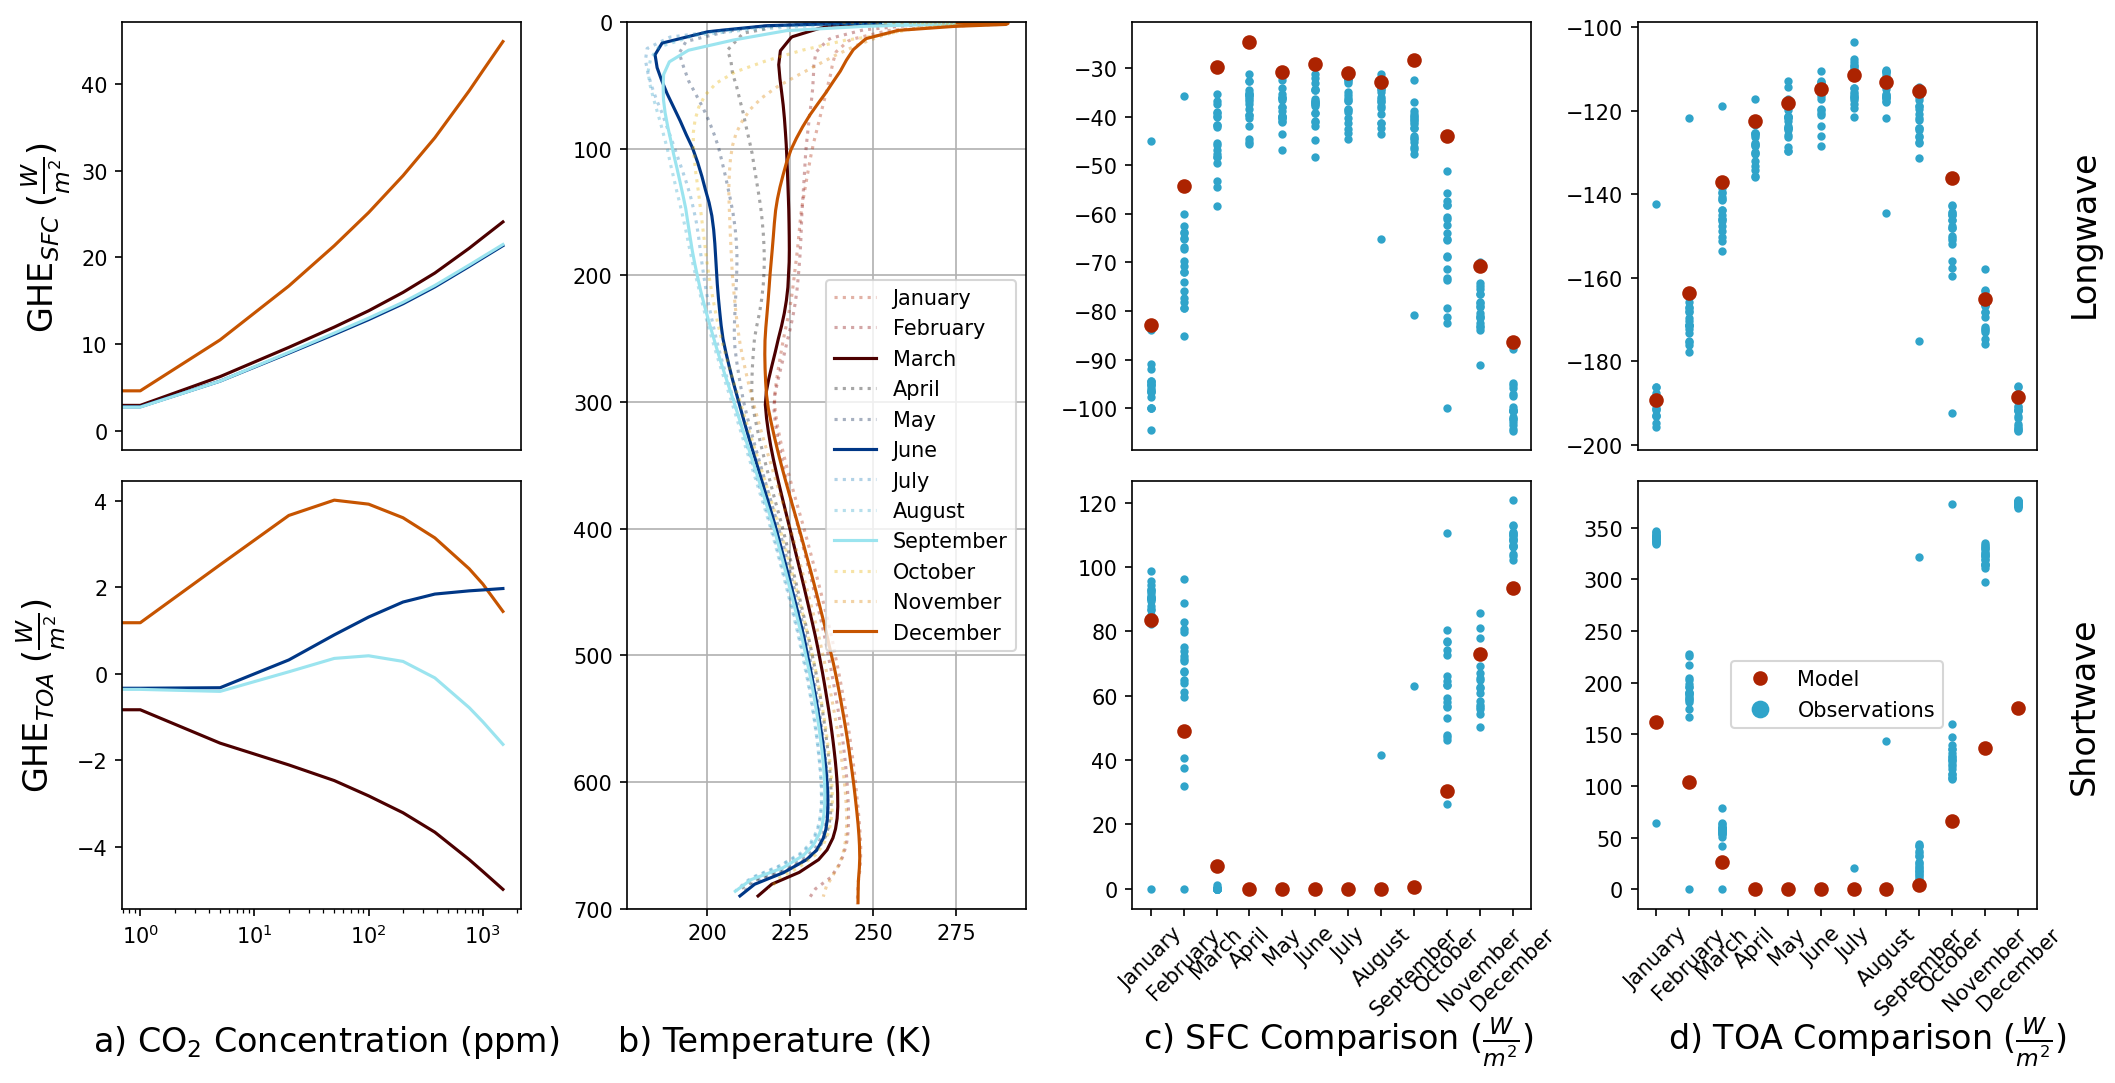
\includegraphics[width=1\textwidth]{figures/GH_sfc_CO2_effect.png}
\centering
\caption{$\text{GHE}_{\text{SFC}}$ (upper) and $\text{GHE}_{\text{TOA}}$ (lower) for a range of \ce{CO_2} concentrations. $\text{GHE}_{\text{SFC}}$ is increasingly positive with higher \ce{CO_2} concentrations, while the responses for $\text{GHE}_{\text{TOA}}$ vary by season.}
\label{fig:sfc_toa_GHE}
\end{figure}

These calculations show that ${\text{GHE}_\text{{SFC}}}$ is always positive, independent of the time of year, while the sign of ${\text{GHE}_\text{{TOA}}}$ is seasonally dependent (Figure \ref{fig:sfc_toa_GHE}). This agrees with the conclusions of previous work  \cite{schmithusen_how_2015}, as we find $\frac{\delta{\text{GHE}_\text{{TOA}}}}{\delta\ce{CO_2}}$ is positive during austral winter months (May-August), but negative throughout the rest of the year (September-April). This increase in OLR with higher \ce{CO_2} concentrations leads to increasing top-of-atmosphere (TOA) radiative loss under higher GHG scenarios during September-April. 

In contrast to this varying response at the TOA, we find that the ${\text{GHE}_\text{{SFC}}}$ is positive across all seasons, and considerably larger in magnitude. Given this consistent response and previous work that has shown surface temperature warming throughout the year in response to CFCs \cite{flanner_climate_2018} as well as a quadrupling of \ce{CO_2} \cite{smith_no_2018}, can we devise a simple model to understand both the magnitude of ${\text{GHE}_\text{{SFC}}}$ and the potential surface warming that would result from it? 

We begin by trying to model ${\text{GHE}_\text{{SFC}}}$ as a function of CO$_2$ concentration and temperature. Using reasoning similar to that of \citeA{jeevanjee_analytical_2020}, we attempt to explain the downward radiation at the surface due to CO$_2$ as the product of an effective bandwidth over which the atmospheric column is optically-thick to CO$_2$, $W(C)$, and the Planck function $\pi B(\nu,T_e)$ at a temperature $T_e$ representative of downward emission from the CO$_2$ band, at frequency $\nu$. Unlike the situation in \citeA{jeevanjee_analytical_2020} where upward TOA fluxes are considered, and different parts of the CO$_2$ band emit to space from different heights and thus at different temperatures, considering downward emission at the surface only requires thinking about downward emission from the air very close to the surface. This simplification occurs because once the atmospheric column is optically thick to CO$_2$ at a given frequency, the effective height for emission to the surface lies very close to the ground, and remains at nearly the same height as CO$_2$ concentrations increase further. Thus, using the surface temperature $T_s$ as a proxy for the temperature at the downward emission, $T_e$, height to the surface, we can write:
\begin{equation}
    {\text{GHE}_\text{{SFC}}} \approx W(C)\times \pi B(\nu,T_s) \label{eq:ghe_sfc}
\end{equation}

We can then estimate the CO$_2$ bandwidth based on equation 7 from \citeA{jeevanjee_analytical_2020} as
\begin{equation}\label{eq:bandwidth}
    W(C) \approx 2\ell ln(\frac{C}{C_0})
\end{equation}
Our Planck function is based on a centered absorption band ($\nu$) of \ce{CO_2} at 667 cm$^-1$, $C_0$ is set to .25 ppmv, $\ell$, the spectroscopic decay parameter, is 10.4 cm$^{-1}$, and C is the \ce{CO_2} concentration. 

The surface greenhouse effect of CO$_2$ is captured well by Equation \ref{eq:ghe_sfc} (Figure \ref{fig:sfc_bandwidth_co2}). The surface greenhouse effect scales nearly logarithmically with CO$_2$ concentration for each month, and when ${\text{GHE}_\text{{SFC}}}$ is divided by the Planck function evaluated at the band center frequency and the surface temperature of each month ($\pi B(\nu,T_s)$) to infer an effective bandwidth, these bandwidths nearly collapse across months (Figure \ref{fig:sfc_bandwidth_co2}). A logarithmic form for the bandwidth slightly overestimates ${\text{GHE}_\text{{SFC}}}$ at lower \ce{CO_2} concentrations, primarily due to overestimation of the bandwidth at low CO$_2$ concentrations. Overall, these calculations indicate that the monotonic increase in ${\text{GHE}_\text{{SFC}}}$ with CO$_2$ concentration can be explained simply as a consequence of downward emission from a CO$_2$ band that widens with increasing CO$_2$, at an emitting temperature close to that of the surface. We expand on this calculation further in section \ref{section:discussion}, by using the functional form of ${\text{GHE}_\text{{SFC}}}$ to explain surface warming with increasing CO$_2$ concentrations in our radiative-advective-turbulent single column model.


\begin{figure}[htb!]
\noindent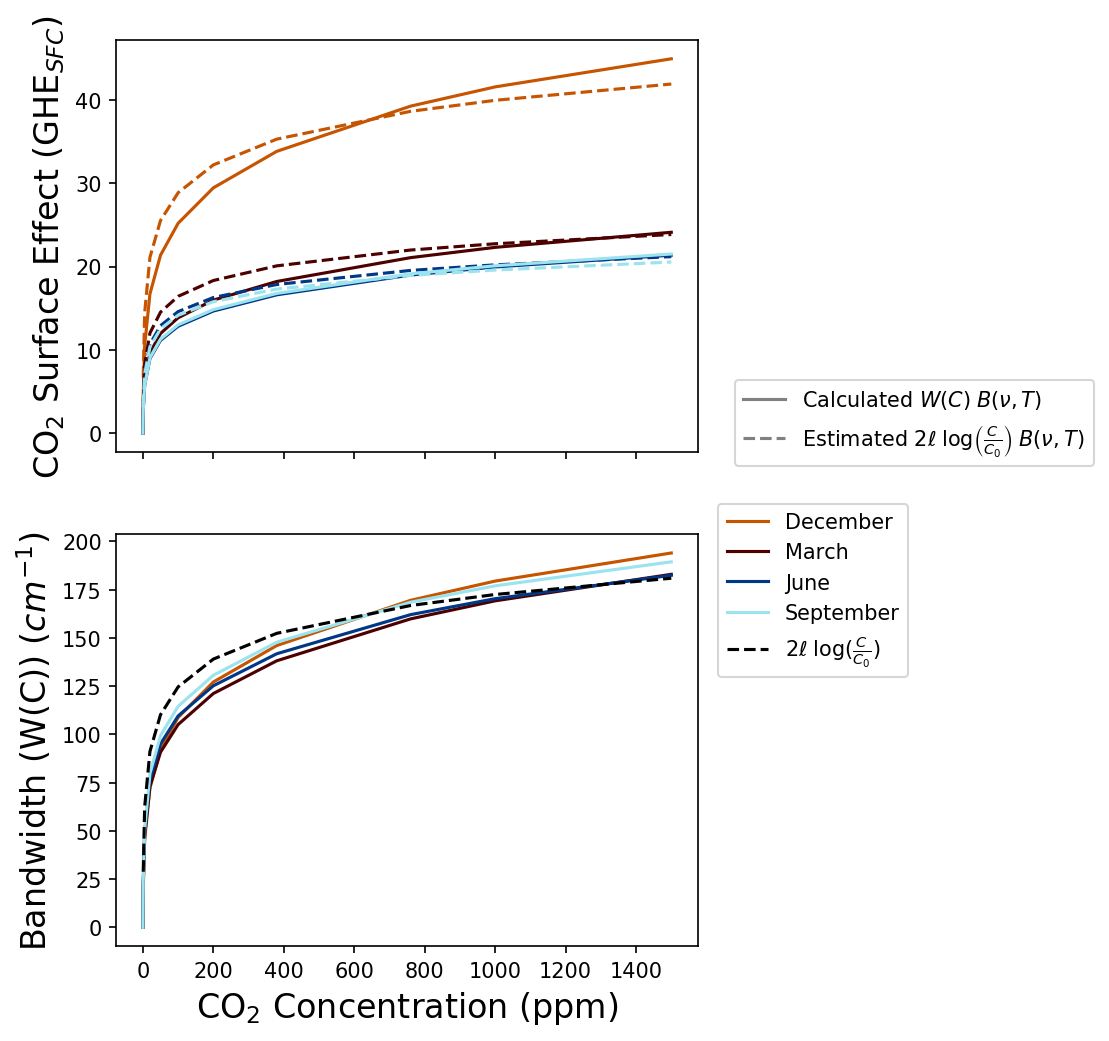
\includegraphics[width=1\textwidth]{figures/sfc_bandwidth_and_co2.png}
\centering
\caption{\ce{CO_2} surface effect (upper) and bandwidth (lower) across varying \ce{CO_2} concentrations from 0-1500 ppm for December, March, June and September. The \ce{CO_2} surface effect is calculated according to equation \ref{eq:ghe_sfc} (solid lines) as well as replacing the bandwidth in Equation \ref{eq:ghe_sfc} with Equation \ref{eq:bandwidth} (dashed lines). The bandwidth is similarly calculated based on \ref{eq:ghe_sfc} (solid lines), and estimated by \ref{eq:bandwidth} (dashed line).}
\label{fig:sfc_bandwidth_co2}
\end{figure}


\section{Radiative-Advective-Turbulent Model}
% Radiative-advective-turbulent calculations - methods + results (surface exchange + advection + time stepping all need to be documented)
% 3) \Delta T (2xCO2 - 1xCO2) for all months with sub-panels for surface T change

We build on the radiative calculations performed above, creating a single column radiative-advective-turbulent model that we run to an equilibrium state. This model computes temperature tendencies from the flux divergence ($\nabla \cdot \mathcal{F}$) of each of the three components and steps the temperature forward in time according to:
\begin{equation}
    \rho c_{p} \frac{\partial T}{\partial t} = -\nabla \cdot \mathbf{\mathcal{F}}.
\end{equation}
The radiation component is calculated as described above using RRTMG, and the turbulent and advective components are added in order to represent turbulence in the planetary boundary layer and meridional advection. Below we describe the development of the turbulent and advective components of the model.

\subsection{Turbulence}
A two-way balance between radiative cooling and advective heating can generate equilibrium temperature profiles, but by construction these have zero turbulent heat flux at the surface, no net surface radiative flux, and a discontinuous temperature jump between the surface and overlying air \cite{cronin_analytic_2016}. Much of the Antarctic plateau has a strong but not discontinuous surface inversion, where surface radiative cooling is balanced by a downward flux of sensible heat from the warmer air above. To capture this transport of heat by boundary-layer turbulence, we include a near-surface turbulent heating component based on the eddy diffusion of potential temperature,
\begin{equation}
    F_{turb} = -k(z) \frac{d\theta}{dz}.
\end{equation}
Here, $k(z) = \overline{k_0} \exp(-\frac{z}{d})$ is an exponentially decaying eddy diffusivity for sensible heat, with a surface value of $k_0$ and a height scale of $d = 100$ meters, which confines turbulent fluxes to the bottom few model levels. To obtain eddy diffusivity values consistent with observed temperature profiles, we first diagnose $k_0$ from the initial temperature profiles for each month $m$,
\begin{equation}
    k_0^{(m)} = \frac{F_{\text{sfc, rad}}}{\frac{d\theta}{dz}_{\text{sfc}}},
\end{equation}
where our radiative surface flux is calculated as
\begin{equation}
    F_{\text{sfc, rad}} = F_{\text{sfc, SW}} - F_{\text{sfc, LW}}.
\end{equation}
From this, we average the (nine) positive values of $k_0^{(m)}$, and use this as our final $\overline{k_0} = 0.423$ throughout the experiments.

The turbulent heating rate is then the flux divergence divided by the heat capacity of air and ice, for the atmosphere and surface, respectively:
\begin{equation}
    \text{HR}_{\text{turb}} = -\frac{dF_{\text{turb}}}{dz} /(c_p \rho).
\end{equation}

This parameterization of turbulent sensible heat fluxes warms the surface in the winter and cools it in the summer, balancing the surface radiative heating rate in equilibrium.

\subsection{Advection}
We calculate our advective heating rate based on the initial state for each month at \ce{CO_2} = 380ppm, where it is set to balance the sum of the radiative and turbulent heating rates.

\begin{equation}
    \frac{dF_{adv}}{dy} = -\left( \frac{dF_{rad}}{dz} + \frac{dF_{turb}}{dz} \right)\quad \text{at t = 0 and \ce{CO_2} = 380 ppm}
\end{equation}
The resulting advective heating rate profile is fixed for each month, in order to allow us to examine how a thermally balanced state with a fixed advective heating rate responds to a perturbation in GHGs. 
\subsection{Equilibrium State}
We run the model forward for five months to assess the equilibrium state in our base and doubled \ce{CO_2} scenarios. Doubling CO$_2$ warms the surface by 1.0-1.4 degrees, but cools the stratosphere dramatically (Figure \ref{fig:temp_dif})  -- the latter effect is expected based on previous work \cite{manabe_thermal_1967,langematz_thermal_2003}. Both this stratospheric cooling and surface temperature warming due to increases in \ce{CO_2} resemble the CO$_2$-induced warming in regions without temperature inversions, and the surface temperature changes fall within similar ranges to those found in \citeA{manabe_thermal_1967} with fixed absolute humidity. Surface warming, despite a negative top-of-atmosphere radiative forcing from CO$_2$ supports previous conclusions by \citeA{smith_no_2018} and \citeA{flanner_climate_2018}. The vertical structure of temperature change -- largest near the surface and with small values throughout much of the troposphere -- differs strongly from that expected in response to CO$_2$ in the tropics, where warming is expected to be greatest in the upper troposphere \cite{fu_warming_2011}.

\begin{figure}[htb!]
\noindent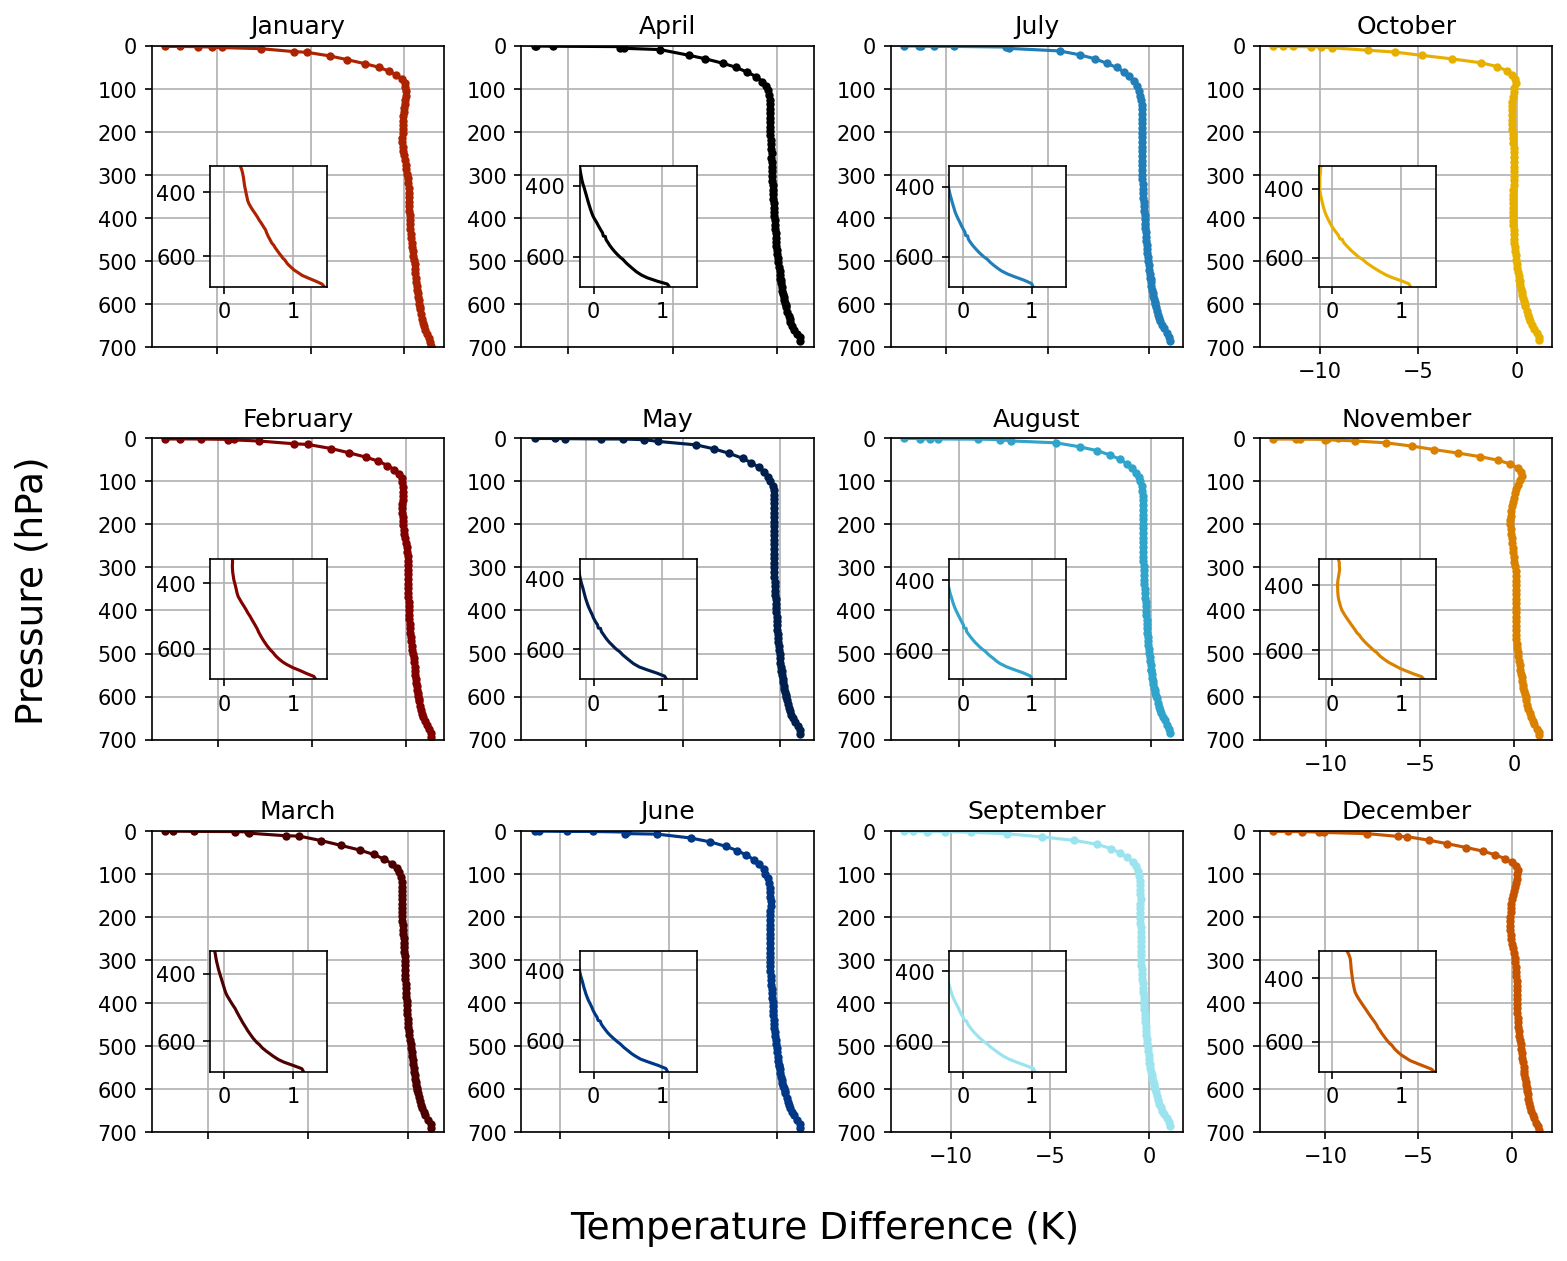
\includegraphics[width=1\textwidth]{figures/temp_dif.png}
\centering
\caption{Vertical profiles of equilibrium temperature differences between the double and base \ce{CO_2} scenario for each month resulting from our model. Insets show changes for the bottom 300 hPa of the atmosphere to highlight the surface warming across all months.}
\label{fig:temp_dif}
\end{figure}


\section{Discussion and Conclusion}\label{section:discussion} 
%
% Discussion 
% 4) predicted surface temperature change (relative to no CO2) compared to radiative-advective-turbulent model calculations (scatter plot)

Is there a simple way to understand the surface temperature change resulting from varying \ce{CO_2} in our simulations? Relative to a situation with no CO$_2$, and considering the perturbation surface radiative energy balance only, $\text{GHE}_\text{{SFC}}$ must be balanced by the additional upward longwave radiation from this warmer surface: $ 4 \sigma T_s^3 \delta T_s = \text{GHE}_{\text{SFC}}$, where $\delta T_s$ is the surface temperature change relative to a simulation with no CO$_2$. We can further simplify this by expressing the CO$_2$ $\text{GHE}_\text{{SFC}}$ as a function of the estimated bandwidth and Planck function, using our approximation of $\text{GHE}_\text{{SFC}}$ from equation \ref{eq:ghe_sfc}. Solving for $\delta T_s$ we find:

\begin{equation}\label{eq:del_ts_planck}
    \delta T_s = \frac{2\ell log(\frac{C}{C_0}) \times \pi B(\nu, T_s)}{4\sigma T_s^3}
\end{equation}

The surface temperature increases due to CO$_2$ across a range of CO$_2$ concentrations and is predicted well by this expression (two months representing different seasons are shown in Figure \ref{fig:delta_ts}). The estimation from equation \ref{eq:del_ts_planck} allows us to calculate the change in temperature due to increasing CO$_2$ based only on the knowledge of an initial temperature state. It may be a surprise that this estimate works well even though the surface is not in radiative equilibrium, and turbulent fluxes can and do change with surface warming. The key, however, is that the turbulent fluxes vanish only a small distance above the surface. Thus, the coupled boundary layer and surface system -- with its top at a level where turbulent fluxes vanish -- can only lose heat by upward radiation, and must warm in order to compensate for an increase in downward longwave fluxes from higher CO$_2$ concentrations.  

Using a radiative-advective-turbulent single column model, we are able to establish a relationship between the surface temperature changes in the Antarctic and the surface radiative forcing across multiple \ce{CO_2} concentrations. The \ce{CO_2} surface greenhouse effect, $\text{GHE}_\text{{SFC}}$, is positive across all months, as is $\frac{\delta{\text{GHE}_\text{{SFC}}}}{\delta\ce{CO_2}}$. In contrast to the $\text{GHE}_\text{{TOA}}$ impacts of changing \ce{CO_2} concentrations, this framework allows for a simple calculation of the change in surface temperature based only on an initial surface temperature, and change in \ce{CO_2} concentration. As in \citeA{flanner_climate_2018}, we find that increased GHG concentrations lead to warming at the Antarctic surface regardless of the sign of the top-of-atmosphere radiative forcing. Our simple calculation could prove helpful to quantifying the specific role of \ce{CO_2} in Antarctic temperature change, complimenting efforts to understand the impacts of GHG, ozone, atmospheric dynamics, and other impacts on Antarctic temperatures \cite{shindell_southern_2004, thompson_signatures_2011}.

\begin{figure}[htb!]
\noindent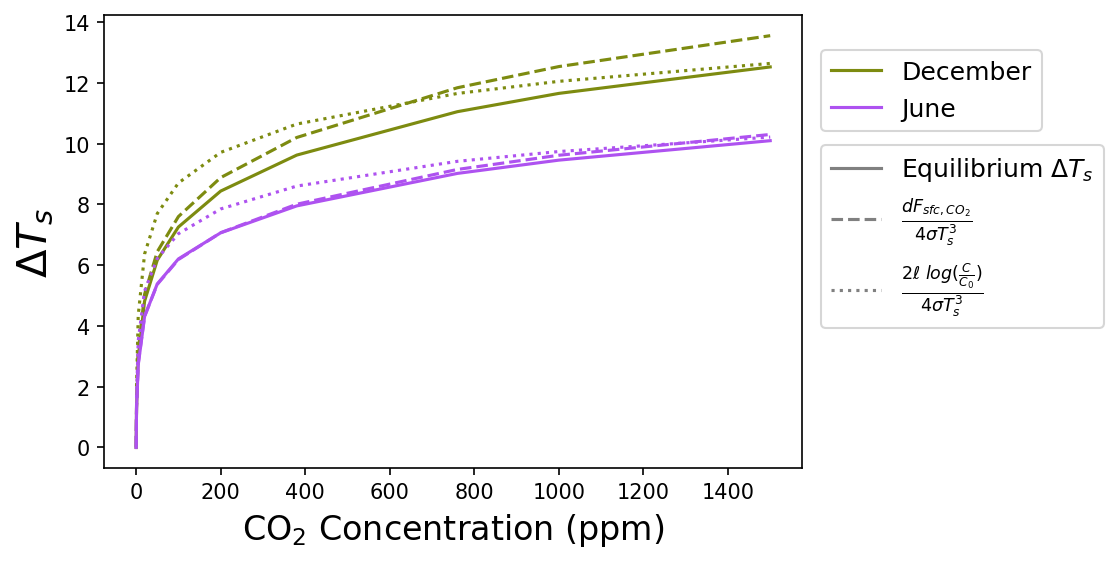
\includegraphics[width=1\textwidth]{figures/delta_Ts.png}
\centering
\caption{Surface temperature change from the initial to equilibrium state for the months of June and December across different \ce{CO_2} values, ranging from 0-1500 ppm, normalized to the 0 ppm T$_s$. The solid lines depict the difference between the initial and equilibrium surface temperature from our single column model; dashed lines indicate the estimated temperature difference based on the derivative of the Stefan-Boltzmann law and the calculated CO$_2$ surface greenhouse effect; dotted lines indicate the estimated temperature difference based on equation \ref{eq:del_ts_planck}. Estimations from equation \ref{eq:del_ts_planck} overestimate at low \ce{CO_2} concentrations, while accuracy of estimations from the Stefan-Boltzmann law vary based on the season.}
\label{fig:delta_ts}
\end{figure}

%%

%  Numbered lines in equations:
%  To add line numbers to lines in equations,
%  \begin{linenomath*}
%  \begin{equation}
%  \end{equation}
%  \end{linenomath*}



%% Enter Figures and Tables near as possible to where they are first mentioned:
%
% DO NOT USE \psfrag or \subfigure commands.
%
% Figure captions go below the figure.
% Table titles go above tables;  other caption information
%  should be placed in last line of the table, using
% \multicolumn2l{$^a$ This is a table note.}
%
%----------------
% EXAMPLE FIGURES
%
% \begin{figure}
% \includegraphics{example.png}
% \caption{caption}
% \end{figure}
%
% Giving latex a width will help it to scale the figure properly. A simple trick is to use \textwidth. Try this if large figures run off the side of the page.
% \begin{figure}
% \noindent\includegraphics[width=\textwidth]{anothersample.png}
%\caption{caption}
%\label{pngfiguresample}
%\end{figure}
%
%
% If you get an error about an unknown bounding box, try specifying the width and height of the figure with the natwidth and natheight options. This is common when trying to add a PDF figure without pdflatex.
% \begin{figure}
% \noindent\includegraphics[natwidth=800px,natheight=600px]{samplefigure.pdf}
%\caption{caption}
%\label{pdffiguresample}
%\end{figure}
%
%
% PDFLatex does not seem to be able to process EPS figures. You may want to try the epstopdf package.
%

%
% ---------------
% EXAMPLE TABLE
%
% \begin{table}
% \caption{Time of the Transition Between Phase 1 and Phase 2$^{a}$}
% \centering
% \begin{tabular}{l c}
% \hline
%  Run  & Time (min)  \\
% \hline
%   $l1$  & 260   \\
%   $l2$  & 300   \\
%   $l3$  & 340   \\
%   $h1$  & 270   \\
%   $h2$  & 250   \\
%   $h3$  & 380   \\
%   $r1$  & 370   \\
%   $r2$  & 390   \\
% \hline
% \multicolumn{2}{l}{$^{a}$Footnote text here.}
% \end{tabular}
% \end{table}

%% SIDEWAYS FIGURE and TABLE
% AGU prefers the use of {sidewaystable} over {landscapetable} as it causes fewer problems.
%
% \begin{sidewaysfigure}
% \includegraphics[width=20pc]{figsamp}
% \caption{caption here}
% \label{newfig}
% \end{sidewaysfigure}
%
%  \begin{sidewaystable}
%  \caption{Caption here}
% \label{tab:signif_gap_clos}
%  \begin{tabular}{ccc}
% one&two&three\\
% four&five&six
%  \end{tabular}
%  \end{sidewaystable}

%% If using numbered lines, please surround equations with \begin{linenomath*}...\end{linenomath*}
%\begin{linenomath*}
%\begin{equation}
%y|{f} \sim g(m, \sigma),
%\end{equation}
%\end{linenomath*}

%%% End of body of article

%%%%%%%%%%%%%%%%%%%%%%%%%%%%%%%%
%% Optional Appendix goes here
%
% The \appendix command resets counters and redefines section heads
%
% After typing \appendix
%
%\section{Here Is Appendix Title}
% will show
% A: Here Is Appendix Title
%
%\appendix
%\section{Here is a sample appendix}

%%%%%%%%%%%%%%%%%%%%%%%%%%%%%%%%%%%%%%%%%%%%%%%%%%%%%%%%%%%%%%%%
%
% Optional Glossary, Notation or Acronym section goes here:
%
%%%%%%%%%%%%%%
% Glossary is only allowed in Reviews of Geophysics
%  \begin{glossary}
%  \term{Term}
%   Term Definition here
%  \term{Term}
%   Term Definition here
%  \term{Term}
%   Term Definition here
%  \end{glossary}

%
%%%%%%%%%%%%%%
% Acronyms
%   \begin{acronyms}
%   \acro{Acronym}
%   Definition here
%   \acro{EMOS}
%   Ensemble model output statistics
%   \acro{ECMWF}
%   Centre for Medium-Range Weather Forecasts
%   \end{acronyms}

%
%%%%%%%%%%%%%%
% Notation
%   \begin{notation}
%   \notation{$a+b$} Notation Definition here
%   \notation{$e=mc^2$}
%   Equation in German-born physicist Albert Einstein's theory of special
%  relativity that showed that the increased relativistic mass ($m$) of a
%  body comes from the energy of motion of the body—that is, its kinetic
%  energy ($E$)—divided by the speed of light squared ($c^2$).
%   \end{notation}




%%%%%%%%%%%%%%%%%%%%%%%%%%%%%%%%%%%%%%%%%%%%%%%%%%%%%%%%%%%%%%%%
%
%  ACKNOWLEDGMENTS
%
% The acknowledgments must list:
%
% >>>>	A statement that indicates to the reader where the data
% 	supporting the conclusions can be obtained (for example, in the
% 	references, tables, supporting information, and other databases).
%
% 	All funding sources related to this work from all authors
%
% 	Any real or perceived financial conflicts of interests for any
%	author
%
% 	Other affiliations for any author that may be perceived as
% 	having a conflict of interest with respect to the results of this
% 	paper.
%
%
% It is also the appropriate place to thank colleagues and other contributors.
% AGU does not normally allow dedications.


\acknowledgments
All data, code needed to run the single column model, and code to re-produce figures from the paper are available at: https://github.com/lfreese/antarctic-rad. 


%% ------------------------------------------------------------------------ %%
%% References and Citations

%%%%%%%%%%%%%%%%%%%%%%%%%%%%%%%%%%%%%%%%%%%%%%%
%
% \bibliography{<name of your .bib file>} don't specify the file extension
%
% don't specify bibliographystyle
%%%%%%%%%%%%%%%%%%%%%%%%%%%%%%%%%%%%%%%%%%%%%%%

\bibliography{references.bib}



%Reference citation instructions and examples:
%
% Please use ONLY \cite and \citeA for reference citations.
% \cite for parenthetical references
% ...as shown in recent studies (Simpson et al., 2019)
% \citeA for in-text citations
% ...Simpson et al. (2019) have shown...
%
%
%...as shown by \citeA{jskilby}.
%...as shown by \citeA{lewin76}, \citeA{carson86}, \citeA{bartoldy02}, and \citeA{rinaldi03}.
%...has been shown \cite{jskilbye}.
%...has been shown \cite{lewin76,carson86,bartoldy02,rinaldi03}.
%... \cite <i.e.>[]{lewin76,carson86,bartoldy02,rinaldi03}.
%...has been shown by \cite <e.g.,>[and others]{lewin76}.
%
% apacite uses < > for prenotes and [ ] for postnotes
% DO NOT use other cite commands (e.g., \citet, p, \citeyear, \nocite, \citealp, etc.).
%



\end{document}



More Information and Advice:

%% ------------------------------------------------------------------------ %%
%
%  SECTION HEADS
%
%% ------------------------------------------------------------------------ %%

% Capitalize the first letter of each word (except for
% prepositions, conjunctions, and articles that are
% three or fewer letters).

% AGU follows standard outline style; therefore, there cannot be a section 1 without
% a section 2, or a section 2.3.1 without a section 2.3.2.
% Please make sure your section numbers are balanced.
% ---------------
% Level 1 head
%
% Use the \section{} command to identify level 1 heads;
% type the appropriate head wording between the curly
% brackets, as shown below.
%
%An example:
%\section{Level 1 Head: Introduction}
%
% ---------------
% Level 2 head
%
% Use the \subsection{} command to identify level 2 heads.
%An example:
%\subsection{Level 2 Head}
%
% ---------------
% Level 3 head
%
% Use the \subsubsection{} command to identify level 3 heads
%An example:
%\subsubsection{Level 3 Head}
%
%---------------
% Level 4 head
%
% Use the \subsubsubsection{} command to identify level 3 heads
% An example:
%\subsubsubsection{Level 4 Head} An example.
%
%% ------------------------------------------------------------------------ %%
%
%  IN-TEXT LISTS
%
%% ------------------------------------------------------------------------ %%
%
% Do not use bulleted lists; enumerated lists are okay.
% \begin{enumerate}
% \item
% \item
% \item
% \end{enumerate}
%
%% ------------------------------------------------------------------------ %%
%
%  EQUATIONS
%
%% ------------------------------------------------------------------------ %%

% Single-line equations are centered.
% Equation arrays will appear left-aligned.

%Math coded inside display math mode \[ ...\]
% will not be numbered, e.g.,:
% \[ x^2=y^2 + z^2\]

 %Math coded inside \begin{equation} and \end{equation} will
% be automatically numbered, e.g.,:
 %\begin{equation}
 %x^2=y^2 + z^2
 %\end{equation}


% To create multiline equations, use the
% \begin{eqnarray} and \end{eqnarray} environment
% as demonstrated below.
%\begin{eqnarray}
 % x_{1} & = & (x - x_{0}) \cos \Theta \nonumber \\
  %      && + (y - y_{0}) \sin \Theta  \nonumber \\
  %y_{1} & = & -(x - x_{0}) \sin \Theta \nonumber \\
  %      && + (y - y_{0}) \cos \Theta.
%\end{eqnarray}

%If you don't want an equation number, use the star form:
%\begin{eqnarray*}...\end{eqnarray*}

% Break each line at a sign of operation
% (+, -, etc.) if possible, with the sign of operation
% on the new line.

% Indent second and subsequent lines to align with
% the first character following the equal sign on the
% first line.

% Use an \hspace{} command to insert horizontal space
% into your equation if necessary. Place an appropriate
% unit of measure between the curly braces, e.g.
% \hspace{1in}; you may have to experiment to achieve
% the correct amount of space.


%% ------------------------------------------------------------------------ %%
%
%  EQUATION NUMBERING: COUNTER
%
%% ------------------------------------------------------------------------ %%

% You may change equation numbering by resetting
% the equation counter or by explicitly numbering
% an equation.

% To explicitly number an equation, type \eqnum{}
% (with the desired number between the brackets)
% after the \begin{equation} or \begin{eqnarray}
% command.  The \eqnum{} command will affect only
% the equation it appears with; LaTeX will number
% any equations appearing later in the manuscript
% according to the equation counter.
%

% If you have a multiline equation that needs only
% one equation number, use a \nonumber command in
% front of the double backslashes (\\) as shown in
% the multiline equation above.

% If you are using line numbers, remember to surround
% equations with \begin{linenomath*}...\end{linenomath*}

%  To add line numbers to lines in equations:
%  \begin{linenomath*}
%  \begin{equation}
%  \end{equation}
%  \end{linenomath*}



